\subsubsection{25.03.15}
\begin{enumerate}
	
	\item The time of beginning and ending of the meeting: 10:00 - 23:59.
	
	\item Purposes of the meeting: 
	\begin{enumerate}
		
		\item Make new strong mechanism of overturning of the bucket.
		
		\item Make blades for gripper for balls.
		
        \item Make ramp for guiding balls into the bucket.
        
        \item Finish working on plexiglass protection.
        
        \item Create a poster for the nomination "Compass Award".
        
        \item Prepare the robot for the flight to the competition.
		
	\end{enumerate}

	\item Work that has been done:
	\begin{enumerate}
		
		\item Today we bought the L-profile and started creating the mechanism of overturning of the bucket.
		
		\item We created new blades for the gripper for balls. As now it became wider, as the material for blades we used a 5-loter plastic bottle. To make blades stronger we infixed them in attaching to the axis with sheets of steel.
		\begin{figure}[H]
			\begin{minipage}[h]{0.2\linewidth}
				\center  
			\end{minipage}
			\begin{minipage}[h]{0.6\linewidth}
				\center{
\includegraphics[scale=0.23]{days/25.03.15/images/01}}
				\caption{}
			\end{minipage}
		\end{figure}
		
        \item After we finished working on gripper for balls, we installed ramp, which guids balls into the bucket. The angle between the floor and the ramp amounted to 77.5${\textdegree}$, so balls fly from the gripper straight up and can be scored into the bucket even though it slightly raised. We were satisfied with these results.
        \begin{figure}[H]
	  	  \begin{minipage}[h]{0.2\linewidth}
	  	    \center  
	  	  \end{minipage}
	  	  \begin{minipage}[h]{0.6\linewidth}
	  		\center{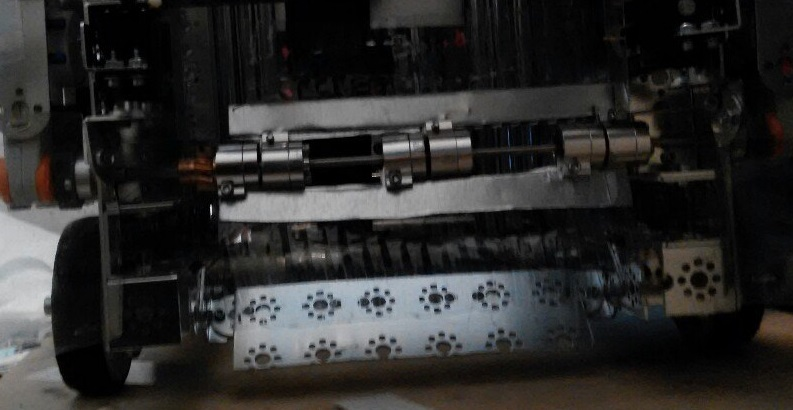
\includegraphics[scale=0.3]{days/25.03.15/images/02}}
	  		\caption{}
	  	  \end{minipage}
	   \end{figure}
	   
	   \item We made the second sheet of plexiglass protection - for the right side of the robot. We also made holes for screws in both sheets of plexiglass.
	   
	   \item Next we installed extra catch for rolling goals to its previous position. To remove extra load from servo we decided to connect it to catching beam with gears. After that we made in the plexiglass protection hole for this gripper.
	   \begin{figure}[H]
	   	\begin{minipage}[h]{0.2\linewidth}
	   		\center  
	   	\end{minipage}
	   	\begin{minipage}[h]{0.6\linewidth}
	   		\center{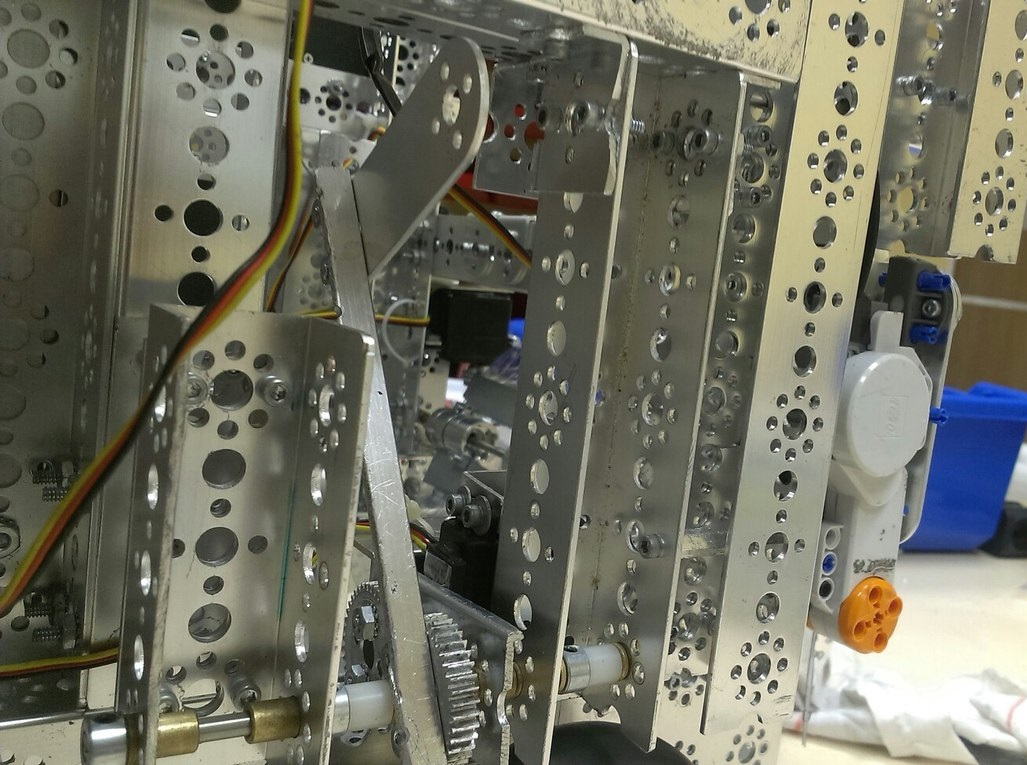
\includegraphics[scale=0.2]{days/25.03.15/images/03}}
	   		\caption{}
	   	\end{minipage}
	   \end{figure}
	   
	   \item Tomorrow we had a flight to Nederlands to the "FTC Dutch Open" competition, so we had to prepare our robot for the transportation. Our robot weighs 18 kg and the box for it - 11 kg. So, in order not to pay for extra weight of the luggage we disassembled robot into modules and put them to different bags.
	   
	   \item Today we created a poster for the nomination "Compass Award" for the competition in Nederlands. For the championship in USA we will make a video for this nomination, but now we don't have any time to do it.
	   
	   \item At the end of the day we printed out our engineering book, stickers for the plexiglass lists, a poster for the "Compass Award" and 150 copies of leaflet with information about our robot (for other teams, judges and guests).

	\end{enumerate}
	
	\item Results:
	\begin{enumerate}
		
		\item Mechanism of overturning of the bucket is not ready yet.
		
		\item Blades for gripper for balls were installed.
		
		\item The ramp for balls was installed.
		
		\item The plexiglass protection is ready.
		
		\item A poster for the nomination "Compass Award" was created.
		
		\item The robot was prepared for the transportation. 
		
	\end{enumerate}
	
	\item Tasks for the next meetings:
	\begin{enumerate}
		
		\item Reassemble robot after a flight.
		
		\item Install the plexiglass protection to the robot and put the stickers onto the plexiglass.
		
        \item Connect servos from the bucket overturner to the controllers.
			
	\end{enumerate}
\end{enumerate}
\fillpage
